\begin{figure}[h!tb]
\centering
%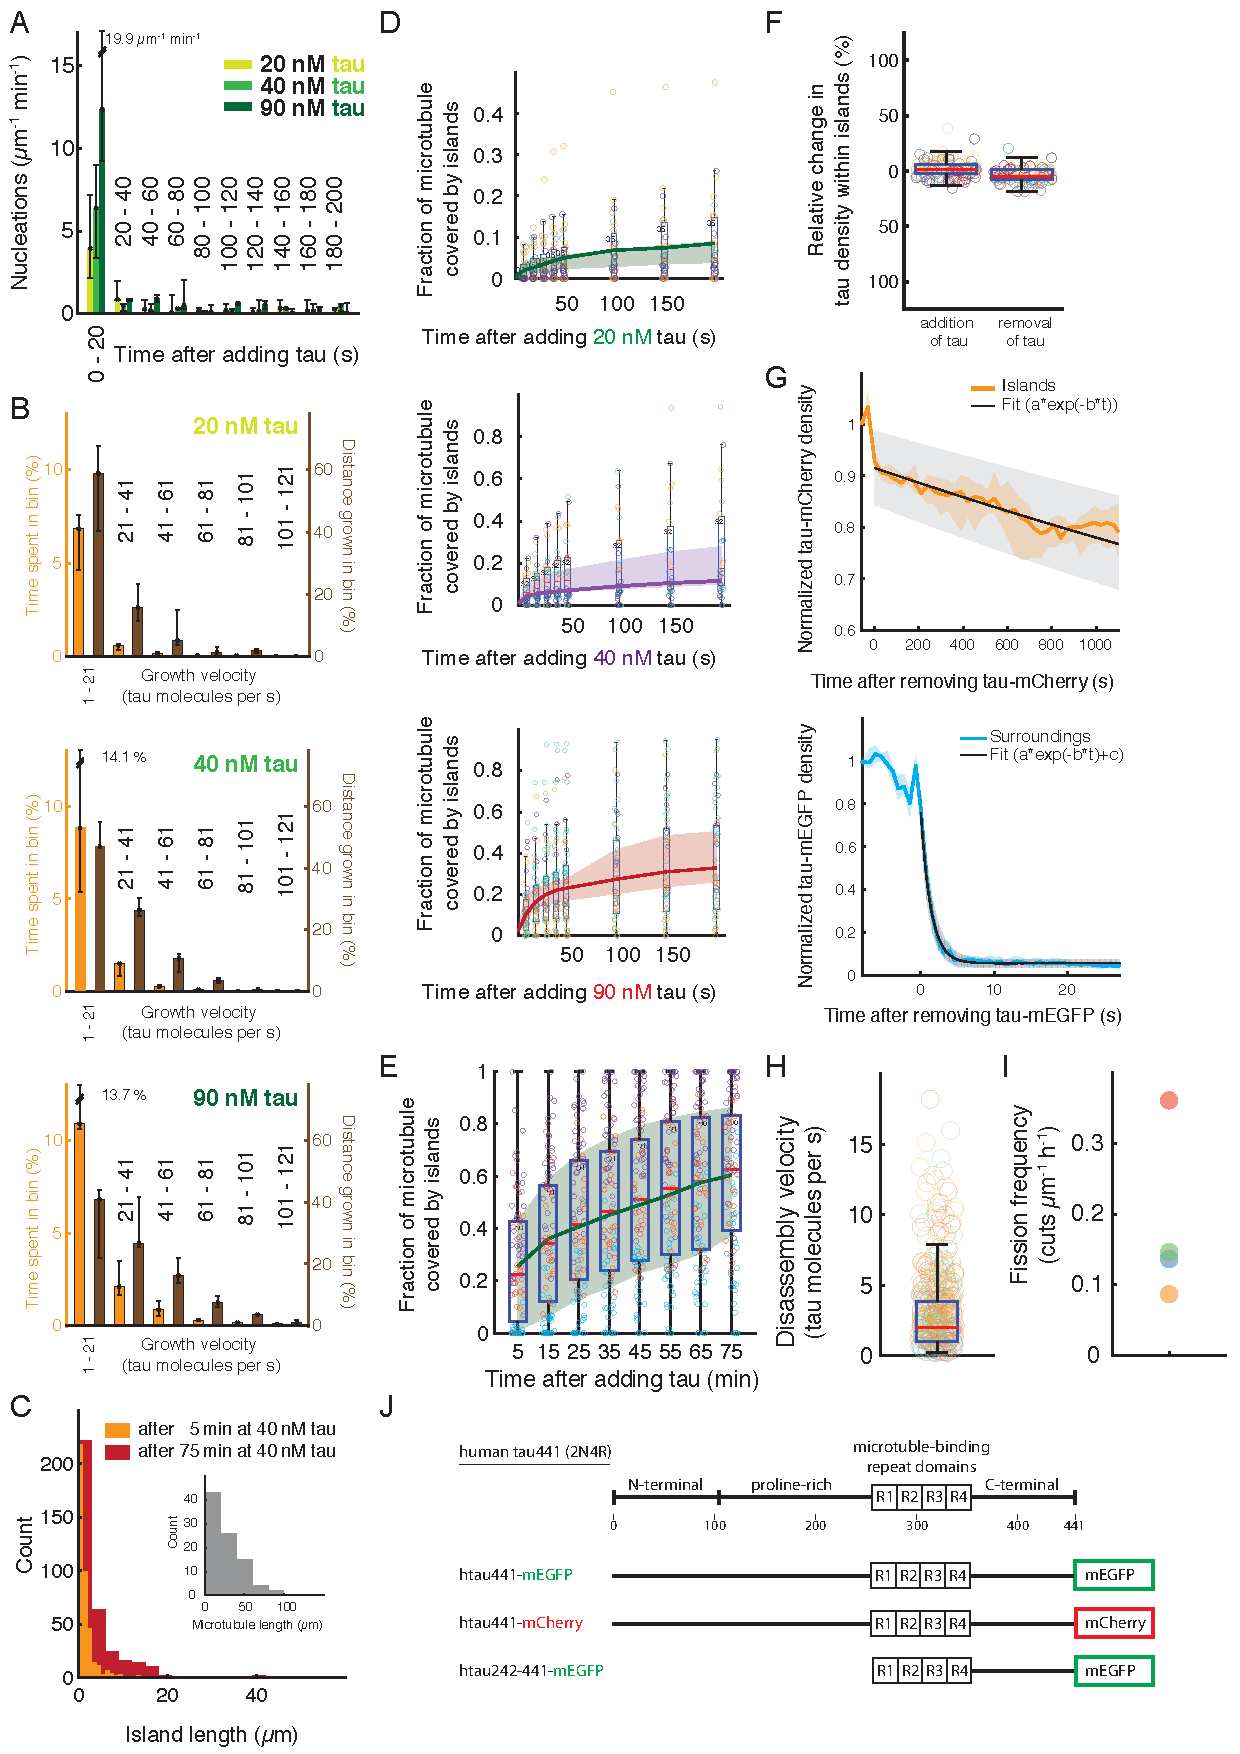
\includegraphics[scale=0.75]{Figures/tau_s1.pdf}
\caption[Supplementary figure for: Tau on microtubules separates into two kinetically distinct phases.]{
Caption on next page.
	}\label{tau_s1}
\end{figure}
\begin{figure}[t]
  \caption{
 (A) Distribution of time between the addition of tau-mEGFP and the formation of the islands (3 experiments per condition, n = 610 nucleation events). Bars show the median; error bars show the minimum and the maximum value. Same experiments as presented in (B) and (D). (B) Histograms of island growth velocities at different tau concentrations in solution (Methods, n = 2131 velocity traces). Same experiments and data representation as in (A). (C) Distribution of the lengths of islands 5 and 75 minutes after the addition of 40 nM tau-mEGFP, n = 91 microtubules in 3 experiments. Distribution of microtubule lengths is shown in the inset. Same experiments as presented in (E). (D) Fraction of microtubule length covered by tau islands at different concentrations of tau-mEGFP in solution. Solid lines and shaded areas (shown also in Figure 1E) represent the median and first and third quartiles values calculated over the whole fields of view (n = 3 experiments). Boxplots represent the same statistics calculated over individual microtubules (n = 40 microtubules for 20 nM tau, n = 32 microtubules for 40 nM tau and n = 59 microtubules for 100 nM tau). The same data as presented in Figure 1E, same experiments as presented in (A). (E) Island assembly does not cease even 75 minutes after the addition of 20 nM tau. The same data representation as in (D), same experiments as presented in (C). (F) Relative difference in tau density within islands i) just after the island nucleation upon the addition of tau and 30 seconds later and ii) just after the removal of tau and 30 seconds later (n = 91 microtubules in 16 experiments). Bleaching was not negligible in the case where tau was absent from solution – for a precise estimation of tau unbinding see (G). (G) Exemplary time-trace of tau-mCherry density inside and tau-mEGFP density outside the islands after removal of tau (mCherry- or mEGFP-labeled, respectively) from solution, analogous to the results presented in Figure 1H (n = 6 microtubules). Single exponential fits are indicated by solid lines. This experiment had been repeated 4 and 3 times for islands and surroundings, respectively, with similar results. Time constants derived from fits for all experiments are shown in Figures 2B and S2D. (H) Distribution of island disassembly velocities upon removal of tau from solution yielding the average velocity of 6.6 ± 5.2 nm/s (average ± SD, corresponding to 2.9 ± 2.3 tau molecules unbinding per second, Methods). Colors encode experiments (n = 335 velocity traces on 90 islands in 4 experiments). For a description of all boxplot elements see Methods. (I) Frequency of fissions occurring within islands upon removal of tau from solution yielding the average 0.20 ± 0.14 fissions per micron of island length per hour (average ± SD). Colors encode n = 4 experiments - same as in (H). (J) Schematics showing the tau constructs used in this study.
  }
\end{figure}
\begin{figure}[h!tb]
\centering
%\includegraphics[scale=0.75]{Figures/tau_s2.png}
\caption[Supplementary figure for: Tau molecules in the islands are stationary but exchange with tau in solution.]{
(A) Exemplary time-trace and fit of tau-mCherry density inside and outside the islands after exchange of 20 nM tau-mCherry for 20 nM tau-mEGFP (n = 5 respectively 7 microtubules). Photo-bleaching during these experiments was negligible (Methods). This experiment had been repeated 5 and 2 times for islands and surroundings, respectively, with similar results. Time constants derived from fits for all experiments are shown in Figures \ref{tau2}C and D. (B) Analogous estimation of tau residence times as in (A) for an exemplary experiment in which 20 nM tau-mCherry was exchanged for 100 nM tau-mEGFP (n = 5 microtubules). The photo-bleaching during this experiment was negligible (Methods). This experiment had been repeated 4 and 2 times for islands and surroundings, respectively, with similar results. Time constants derived from fits for all experiments are shown in Figures \ref{tau2}C and D. (C) Histogram of fluorescence intensities of single tau-mEGFP particles bound to microtubules in experiments as presented in Figure \ref{tau2}E, showing that tau-mEGFP is associated with the microtubule in monomeric form (n = 1861 molecules inside the islands, n = 2210 molecules outside the islands, 1 experiment). (D) Mean square displacement over time of single tau-EGFP molecules inside and outside the islands yielding tau diffusion constants of 0.27 ± 0.15 µm2s-1 (95\% confidence bounds, n = 3660 molecules) outside the islands and 0.027  ± 0.016 µm2s-1 (95\% confidence bounds, n = 2558 molecules, 3 experiments) inside the islands. For comparison, the analogously estimated diffusion constant of non-motile kinesin-1 molecules tightly bound to the microtubule in the presence of AMP-PNP (in the absence of ATP) was 0.014 ± 0.016 µm2s-1 (95\% confidence bounds, n = 126 molecules, 1 experiment).
	}\label{tau_s2}
\end{figure}
\begin{figure}[h!tb]
\centering
%\includegraphics[scale=0.9]{Figures/tau_s4.png}
\caption[Supplementary figure for: Tau islands are distinguished by tau cohesion.]{ (A) Multichannel fluorescence kymograph showing the motion of kip3-GFP (green) inside and outside the tau islands (red). Red arrow indicates the accumulation of kip3-GFP in front of the island. White arrows indicate kip3-GFP molecules speeding up as they leave the island. Scale bar 2 µm. This experiment had been repeated 7 times with similar results. 
	}\label{tau_s4}
\end{figure}
\begin{figure}[h!tb]
\centering
%\includegraphics[scale=0.9]{Figures/tau_s5.png}
\caption[Supplementary figure for: Tau islands are distinguished by tau cohesion.]{
(A) The density of tau-mEGFP on the microtubules saturates at high (µM) tau-mEGFP concentrations (total of 29 and 27 experiments for islands and surroundings, respectively). Horizontal lines indicate the three quartiles. (B) At tau-mEGFP concentrations in the range of 20 nM to approximately 1 µM, the tau-mEGFP density inside the islands scales linearly with the tau-mEGFP density outside the islands. Points indicate medians, error bars indicate the first and third quartiles (both axes). Data from the experiments presented in (A).
	}\label{tau_s5}
\end{figure}

\begin{figure}[h!tb]
\centering
%\includegraphics[scale=0.82]{Figures/tau_s7.png}
\caption[Tau islands do not form at regions of high microtubule curvature.]{
\textbf{Supplementary figure for: Tau islands do not form at regions of high microtubule curvature.} 
(A) Densities of tau-mCherry outside the islands, inside the islands and in the regions of high curvature (after the removal of 0.8 µM tau from solution). Points are color-coded by experiments, horizontal lines indicate the three quartiles, weighted such that each experiment has equal weight. 
(B) Tau density profile along the microtubule after removing 800 nM tau from solution. X-axis is centered on the point of highest curvature. Data are color-coded by microtubule and the density is normalized to the 90th percentile of the density-values of the respective microtubule. The red line represents the median of n = 30 microtubules (7 experiments), the first and third quartile are indicated by the shaded area. At 800 nM tau, there always were islands adjacent to microtubule bends, which is why the tau density to the left and right of the curved microtubule region is high even though tau has been removed from solution. A clear decrease in the tau density is apparent at the point of highest curvature.
(C) Kymograph showing the uniform increase of tau-mEGFP density along the whole region of the microtubule curve upon the addition of tau-mEGFP in solution. This is in strong contrast to islands localized on straight microtubules, which grew at their boundaries. Scale bars, vertical 10 min, horizontal 2 µm.
	}\label{tau_s7}
\end{figure}

